\documentclass[11pt]{article}

% --- Package imports ---
% ------------------ MINIMAL WORKING PAPER ------------------
\usepackage[english]{babel}

\usepackage{amsmath,amsfonts,amsthm,amssymb,mathtools} % Mathematical

\usepackage[dvipsnames]{xcolor}
\usepackage{etoolbox} 
\usepackage{tikz} % Drawings
  \usetikzlibrary{3d}
\usepackage{pgfplots} %Pode plotar
  \pgfplotsset{compat=newest}
  \usepgfplotslibrary{fillbetween}
\usepackage{float} 
\usepackage{multirow} 
\usepackage{natbib} 

% ------------------ EXTRA BUT USEFUL ------------------
\usepackage{optidef} 
\usepackage{blindtext} 

\usepackage{hyperref,theoremref} 
\hypersetup{
    pdftitle={PS - Nícolas},
    colorlinks=true, linkcolor=blue!90,
    bookmarksnumbered=true,
    bookmarksopen=true
}

\usepackage{listings}

\usepackage[paper=portrait,pagesize]{typearea}
\usepackage{hyperref}
\usepackage{dcolumn}
\usepackage{footnote}
\usepackage{ulem}
\usepackage{pdfpages}
\usepackage{graphicx}

% ------------------ EXTRA FOR LECTURE NOTES ------------------
\usepackage{
  dsfont,          % Math typesetting
  wrapfig,                           % Figures and graphics formatting
  color, inconsolata, pythonhighlight,               % Code formatting
  fancyhdr, sectsty, enumerate, enumitem, framed }   % Headers/footers, section fonts, links, lists

% lipsum is just for generating placeholder text and can be removed
\usepackage{hyperref, lipsum} 


\usepackage{newpxtext, newpxmath, inconsolata}
\usepackage{algorithm}
\usepackage{algorithmic}
% ------------------ LETTERFONTS ------------------
% Requires amssymb (or amsfonts,mathtools

% Conjuntos
\newcommand{\CC}[1][]{\ensuremath{\ifstrempty{#1}{\mathbb{C}}{\mathbb{C}^{#1}}}}
\newcommand{\EE}[1][]{\ensuremath{\ifstrempty{#1}{\mathbb{E}}{\mathbb{E}^{#1}}}}
\newcommand{\FF}[1][]{\ensuremath{\ifstrempty{#1}{\mathbb{F}}{\mathbb{F}^{#1}}}}
\newcommand{\HH}[1][]{\ensuremath{\ifstrempty{#1}{\mathbb{H}}{\mathbb{H}^{#1}}}}
\newcommand{\II}[1][]{\ensuremath{\ifstrempty{#1}{\mathbb{I}}{\mathbb{I}^{#1}}}}
\newcommand{\KK}[1][]{\ensuremath{\ifstrempty{#1}{\mathbb{K}}{\mathbb{K}^{#1}}}}
\newcommand{\NN}[1][]{\ensuremath{\ifstrempty{#1}{\mathbb{N}}{\mathbb{N}^{#1}}}}
\newcommand{\PP}[1][]{\ensuremath{\ifstrempty{#1}{\mathbb{P}}{\mathbb{P}^{#1}}}}
\newcommand{\QQ}[1][]{\ensuremath{\ifstrempty{#1}{\mathbb{Q}}{\mathbb{Q}^{#1}}}}
\newcommand{\RR}[1][]{\ensuremath{\ifstrempty{#1}{\mathbb{R}}{\mathbb{R}^{#1}}}}
\newcommand{\ZZ}[1][]{\ensuremath{\ifstrempty{#1}{\mathbb{Z}}{\mathbb{Z}^{#1}}}}

% Letras Blackboard
\newcommand{\bbA}{\ensuremath{\mathbb{A}}}   \newcommand{\bbB}{\ensuremath{\mathbb{B}}}
\newcommand{\bbC}{\ensuremath{\mathbb{C}}}   \newcommand{\bbD}{\ensuremath{\mathbb{D}}}
\newcommand{\bbE}{\ensuremath{\mathbb{E}}}   \newcommand{\bbF}{\ensuremath{\mathbb{F}}}
\newcommand{\bbG}{\ensuremath{\mathbb{G}}}   \newcommand{\bbH}{\ensuremath{\mathbb{H}}}
\newcommand{\bbI}{\ensuremath{\mathbb{I}}}   \newcommand{\bbJ}{\ensuremath{\mathbb{J}}}
\newcommand{\bbK}{\ensuremath{\mathbb{K}}}   \newcommand{\bbL}{\ensuremath{\mathbb{L}}}
\newcommand{\bbM}{\ensuremath{\mathbb{M}}}   \newcommand{\bbN}{\ensuremath{\mathbb{N}}}
\newcommand{\bbO}{\ensuremath{\mathbb{O}}}   \newcommand{\bbP}{\ensuremath{\mathbb{P}}}
\newcommand{\bbQ}{\ensuremath{\mathbb{Q}}}   \newcommand{\bbR}{\ensuremath{\mathbb{R}}}
\newcommand{\bbS}{\ensuremath{\mathbb{S}}}   \newcommand{\bbT}{\ensuremath{\mathbb{T}}}
\newcommand{\bbU}{\ensuremath{\mathbb{U}}}   \newcommand{\bbV}{\ensuremath{\mathbb{V}}}
\newcommand{\bbW}{\ensuremath{\mathbb{W}}}   \newcommand{\bbX}{\ensuremath{\mathbb{X}}}
\newcommand{\bbY}{\ensuremath{\mathbb{Y}}}   \newcommand{\bbZ}{\ensuremath{\mathbb{Z}}}

\newcommand{\bbzero}{\ensuremath{\mathbb{0}}}
\newcommand{\bbone}{\ensuremath{\mathbb{1}}}

% Letras caligráficas
\newcommand{\mcA}{\ensuremath{\mathcal{A}}}  \newcommand{\mcB}{\ensuremath{\mathcal{B}}}
\newcommand{\mcC}{\ensuremath{\mathcal{C}}}  \newcommand{\mcD}{\ensuremath{\mathcal{D}}}
\newcommand{\mcE}{\ensuremath{\mathcal{E}}}  \newcommand{\mcF}{\ensuremath{\mathcal{F}}}
\newcommand{\mcG}{\ensuremath{\mathcal{G}}}  \newcommand{\mcH}{\ensuremath{\mathcal{H}}}
\newcommand{\mcI}{\ensuremath{\mathcal{I}}}  \newcommand{\mcJ}{\ensuremath{\mathcal{J}}}
\newcommand{\mcK}{\ensuremath{\mathcal{K}}}  \newcommand{\mcL}{\ensuremath{\mathcal{L}}}
\newcommand{\mcM}{\ensuremath{\mathcal{M}}}  \newcommand{\mcN}{\ensuremath{\mathcal{N}}}
\newcommand{\mcO}{\ensuremath{\mathcal{O}}}  \newcommand{\mcP}{\ensuremath{\mathcal{P}}}
\newcommand{\mcQ}{\ensuremath{\mathcal{Q}}}  \newcommand{\mcR}{\ensuremath{\mathcal{R}}}
\newcommand{\mcS}{\ensuremath{\mathcal{S}}}  \newcommand{\mcT}{\ensuremath{\mathcal{T}}}
\newcommand{\mcU}{\ensuremath{\mathcal{U}}}  \newcommand{\mcV}{\ensuremath{\mathcal{V}}}
\newcommand{\mcW}{\ensuremath{\mathcal{W}}}  \newcommand{\mcX}{\ensuremath{\mathcal{X}}}
\newcommand{\mcY}{\ensuremath{\mathcal{Y}}}  \newcommand{\mcZ}{\ensuremath{\mathcal{Z}}}

% Letras em negrito

% Letras em negrito
\newcommand{\bfA}{\ensuremath{\mathbf{A}}}   \newcommand{\bfB}{\ensuremath{\mathbf{B}}}
\newcommand{\bfC}{\ensuremath{\mathbf{C}}}   \newcommand{\bfD}{\ensuremath{\mathbf{D}}}
\newcommand{\bfE}{\ensuremath{\mathbf{E}}}   \newcommand{\bfF}{\ensuremath{\mathbf{F}}}
\newcommand{\bfG}{\ensuremath{\mathbf{G}}}   \newcommand{\bfH}{\ensuremath{\mathbf{H}}}
\newcommand{\bfI}{\ensuremath{\mathbf{I}}}   \newcommand{\bfJ}{\ensuremath{\mathbf{J}}}
\newcommand{\bfK}{\ensuremath{\mathbf{K}}}   \newcommand{\bfL}{\ensuremath{\mathbf{L}}}
\newcommand{\bfM}{\ensuremath{\mathbf{M}}}   \newcommand{\bfN}{\ensuremath{\mathbf{N}}}
\newcommand{\bfO}{\ensuremath{\mathbf{O}}}   \newcommand{\bfP}{\ensuremath{\mathbf{P}}}
\newcommand{\bfQ}{\ensuremath{\mathbf{Q}}}   \newcommand{\bfR}{\ensuremath{\mathbf{R}}}
\newcommand{\bfS}{\ensuremath{\mathbf{S}}}   \newcommand{\bfT}{\ensuremath{\mathbf{T}}}
\newcommand{\bfU}{\ensuremath{\mathbf{U}}}   \newcommand{\bfV}{\ensuremath{\mathbf{V}}}
\newcommand{\bfW}{\ensuremath{\mathbf{W}}}   \newcommand{\bfX}{\ensuremath{\mathbf{X}}}
\newcommand{\bfY}{\ensuremath{\mathbf{Y}}}   \newcommand{\bfZ}{\ensuremath{\mathbf{Z}}}

\newcommand{\bfa}{\ensuremath{\mathbf{a}}}   \newcommand{\bfb}{\ensuremath{\mathbf{b}}}
\newcommand{\bfc}{\ensuremath{\mathbf{c}}}   \newcommand{\bfd}{\ensuremath{\mathbf{d}}}
\newcommand{\bfe}{\ensuremath{\mathbf{e}}}   \newcommand{\bff}{\ensuremath{\mathbf{f}}}
\newcommand{\bfg}{\ensuremath{\mathbf{g}}}   \newcommand{\bfh}{\ensuremath{\mathbf{h}}}
\newcommand{\bfi}{\ensuremath{\mathbf{i}}}   \newcommand{\bfj}{\ensuremath{\mathbf{j}}}
\newcommand{\bfk}{\ensuremath{\mathbf{k}}}   \newcommand{\bfl}{\ensuremath{\mathbf{l}}}
\newcommand{\bfm}{\ensuremath{\mathbf{m}}}   \newcommand{\bfn}{\ensuremath{\mathbf{n}}}
\newcommand{\bfo}{\ensuremath{\mathbf{o}}}   \newcommand{\bfp}{\ensuremath{\mathbf{p}}}
\newcommand{\bfq}{\ensuremath{\mathbf{q}}}   \newcommand{\bfr}{\ensuremath{\mathbf{r}}}
\newcommand{\bfs}{\ensuremath{\mathbf{s}}}   \newcommand{\bft}{\ensuremath{\mathbf{t}}}
\newcommand{\bfu}{\ensuremath{\mathbf{u}}}   \newcommand{\bfv}{\ensuremath{\mathbf{v}}}
\newcommand{\bfw}{\ensuremath{\mathbf{w}}}   \newcommand{\bfx}{\ensuremath{\mathbf{x}}}
\newcommand{\bfy}{\ensuremath{\mathbf{y}}}   \newcommand{\bfz}{\ensuremath{\mathbf{z}}}

\newcommand{\bfzero}{\ensuremath{\mathbf{0}}}   \newcommand{\bfone}{\ensuremath{\mathbf{1}}}



% ------------------ COLORS ------------------
% Requires xcolor

%\definecolor{black}{HTML}{212529}
%\definecolor{white}{HTML}{f8f9fa}
%\definecolor{gray}{HTML}{495057}
%\definecolor{red}{HTML}{c92a2a}
%\definecolor{pink}{HTML}{a61e4d}
%\definecolor{grape}{HTML}{862e9c}
%\definecolor{violet}{HTML}{5f3dc4}
%\definecolor{indigo}{HTML}{364fc7}
%\definecolor{blue}{HTML}{1864ab}
%\definecolor{cyan}{HTML}{0b7285}
%\definecolor{teal}{HTML}{087f5b}
%\definecolor{green}{HTML}{2b8a3e}
%\definecolor{lime}{HTML}{5c940d}
%\definecolor{yellow}{HTML}{e67700}
%\definecolor{orange}{HTML}{d9480f}
\definecolor{myBlue}{HTML}{1A476F}
\definecolor{friendlyBlue}{HTML}{1e88e5}
\definecolor{friendlyPink}{HTML}{d81b60}
\definecolor{friendlyYellow}{HTML}{ffc107}
\definecolor{friendlyGreen}{HTML}{409d70}

% ------------------ MACROS ------------------
% Requires tikz, amssymb (or amsfonts), mathtools

% Delimitadores
%\DeclarePairedDelimiter{\abs}{\lvert}{\rvert}
%\DeclarePairedDelimiter{\dotp}{\langle}{\rangle}
%\DeclarePairedDelimiter{\norm}{\lVert}{\rVert}

%\DeclarePairedDelimiter{\ceil}{\lceil}{\rceil}
%\DeclarePairedDelimiter{\floor}{\lfloor}{\rfloor}
%\DeclarePairedDelimiter{\round}{\lfloor}{\rceil}

% Derivadas
\providecommand*{\dv}[3][]{\frac{d^{#1}#2}{d#3^{#1}}}
\providecommand*{\pdv}[3][]{\frac{\partial^{#1}#2}{\partial#3^{#1}}}

% Estatística
\DeclareMathOperator{\var}{Var} % Variância
\DeclareMathOperator{\cov}{Cov} % Covariância

% Menor e Maior ou igual 
\let\oldleq\leq 
\let\oldgeq\geq
\renewcommand{\leq}{\leqslant}
\renewcommand{\geq}{\geqslant}

% Operadores Lógicos
\renewcommand{\iff}{\Leftrightarrow}
\renewcommand{\implies}{\Rightarrow}

\newcommand{\tq}{\text{ tal que }}
\newcommand{\e}{\text{ e }}
\newcommand{\ou}{\text{ ou }}

% Checkmarks
\newcommand{\xmark}{\;%
\tikz[scale=0.23] {
    \draw[line width=0.7,line cap=round,myr] (0,0) to [bend left=6] (1,1);
    \draw[line width=0.7,line cap=round,myr] (0.2,0.95) to [bend right=3] (0.8,0.05);
}}
\renewcommand{\checkmark}{\;%
\tikz[scale=0.23] {
    \draw[line width=0.7,line cap=round,myg] (0.25,0) to [bend left=10] (1,1);
    \draw[line width=0.8,line cap=round,myg] (0,0.35) to [bend right=1] (0.23,0);
}}

% Inverso
\newcommand{\inv}{^{-1}}

% Teoria dos Conjuntos
\DeclareMathOperator{\dom}{D} % Domínio
\DeclareMathOperator{\img}{Im} % Imagem
\DeclareMathOperator{\co}{co} % Convexo

% Álgebra Linear
\DeclareMathOperator{\dist}{d} % Distância
\renewcommand{\det}{\text{det}} % Determinante

% Gregas mais bonitas
\newcommand{\eps}{\epsilon}
\newcommand{\veps}{\varepsilon}
\newcommand{\vphi}{\varphi}

% Sublinhado
\newcommand{\ol}{\overline}
\newcommand{\ul}{\underline}
\newcommand{\ob}{\overbrace}
\newcommand{\ub}{\underbrace}
\newcommand{\wt}{\widetilde}
\newcommand{\wh}{\widehat}

\newcommand{\Qed}{\begin{flushright} \qed \end{flushright}}

\newcommand{\dps}[1]{\displaystyle{#1}}

% Toogle Nico''''
%\renewcommand{\land}{\text{ and }}
%\renewcommand{\lor}{\text{ or }}

% A fazer 
\newcommand\numberthis{\addtocounter{equation}{1}\tag{\theequation}}


% Theorems
\newtheorem{proposition}{Proposition}
\newtheorem{assumption}{Assumption}
\newcommand{\BRL}{\text{R}\$}

%\game: fazer matrix de payoff bonita
\newcounter{nblin}
\newcounter{nbcol}
\newcounter{nbcoltwo}
\newcounter{contest}
\newcounter{contpay}

\newcommand{\gameCell}[2]{({\color{blue} #1},{\color{red} #2})}
\newcommand{\gamePlayer}[2]{{\color{blue} #1}{\color{red} #2}}
\makeatletter
\def\game[#1,#2][#3,#4][#5]{
    \setcounter{nblin}{0}
    \setcounter{nbcol}{0}
    \setcounter{nbcoltwo}{0}
    \setcounter{contest}{0}
    \setcounter{contpay}{0}

    % #1 = Jogador 1
    % #2 = Jogador 2
    % #3 = Estratégias de 1
    % #4 = Estratégias de 2
    % #5 = Matrix de payoffs
    % #6 = bool(0: se sem linhas, 1: com linhas e na diagonal)
    \foreach \j in {#3} {

      \addtocounter{nblin}{1}
    }
    \foreach \j in {#4} {
        \addtocounter{nbcol}{1}
    }
    \addtocounter{nbcol}{2}
    \setcounter{nbcoltwo}{\thenbcol}
    \addtocounter{nbcol}{-2}

    \def\tablehead{%
    \multicolumn{2}{c}{} & \multicolumn{\thenbcol}{c}{{\color{red}\textbf{#2}}}\\\cline{3-\thenbcoltwo} \multicolumn{1}{c}{}&}
    %
        \foreach \lhs in {#4}{
              \protected@xappto\tablehead{ & {\color{red}\textit{\lhs}}}
    }

      %\addtocounter{nbcol}{2}
    %\protected@xappto\tableheader{ \\\cline{3-\thenbcol}}
    %\addtocounter{nbcol}{-2}
    \def\tabledata{\multirow{\thenblin}*{{\color{blue}\textbf{#1}}}}% reset \tabledata

        \setcounter{contest}{0}
        \foreach \j in {#3}{
          \addtocounter{contest}{1}
              \protected@xappto\tabledata{& {\color{blue}\textit{\j}}}
              \setcounter{contpay}{0}
              \foreach \l in {#5}{
                \addtocounter{contpay}{1}
                \ifnum \thecontest=\thecontpay{     
                  \foreach \lhs/\rhs in \l {% build table data from #1
                    \protected@xappto\tabledata{ & {\color{blue}\lhs},\;{\color{red}\rhs}}
                    }
                  \gappto\tabledata{\\}
                }
                \else{}\fi
             }
        }

        \begin{table}[H]
          \centering
          \begin{tabular}{c|c|*{\thenbcol}{c}|}
              \tablehead\\\cline{2-\thenbcoltwo}
              \tabledata\cline{2-\thenbcoltwo}
          \end{tabular}

        \end{table}
}
\makeatother


\newenvironment{economics_diagram}[4]{
\begin{figure}[H]
    \centering
    \begin{tikzpicture}
        \begin{axis}[
              scale only axis, 
              grid=major, 
              grid style={dashed, gray!20},
              %minor x tick num=5,
              %minor y tick num=5,
              axis x line=center,
              axis y line=center, 
              xlabel style={below right},
              ylabel style={above left},
              xmin=0,
              ymin=0,
              xlabel={#1}, %Variável
              ylabel={#2}, %Variável           
              xmax={#3*1.05},  
              ymax={#4*1.05}
              ]
              \path [name path=xaxis]
                      (\pgfkeysvalueof{/pgfplots/xmin},0) --
                      (\pgfkeysvalueof{/pgfplots/xmax},0);
                      
              \pgfplotsset{domain = 0:{#3*1.05}};

        }{
        \end{axis}
    \end{tikzpicture}
\end{figure}
}

\newenvironment{edgeworth_box}[4]{
\begin{figure}[H]
    \centering
    \begin{tikzpicture}
        \begin{axis}[
              scale only axis, 
              grid=major, 
              grid style={dashed, gray,opacity=.2},
              %minor x tick num=5,
              %minor y tick num=5,
              xmin=0,
              ymin=0,
              xlabel={#1}, %Variável
              ylabel={#2}, %Variável           
              xmax={#3},  
              ymax={#4},
              view={0}{90}
              ] 
              \pgfplotsset{domain = 0:{max(#3,#4)*1.05}};
            \addplot[color=black,mark=*,mark size = 1] (0,0) node[above right] {Alice};           
            \addplot[color=black,mark=*,mark size = 1] (#3,#4) node[below left] {Bob};
         
        }{
        \end{axis}
    \end{tikzpicture}
\end{figure}
}


\newcommand{\addLabel}[3]{
    \node at (#1,#2) {\footnotesize #3};
 }

\NewDocumentCommand{\addIC}{O{red}O{red}mm}{
    \addplot3 [
    name path global=#2,
    thick,
    contour gnuplot={
        levels=0,
        labels=false,
        draw color=#1
    },
    samples=25
    ] {#3-(#4)};
}

\NewDocumentCommand{\addPlot}{O{red}O{red}m}{
    \addplot[name path=#1,samples=50,#2,thick,smooth]{#3};
}

\NewDocumentCommand{\addArea}{O{red}mmm}{
    \addplot[#1, opacity=0.2] fill between [of=#2 and #3, soft clip={domain=#4}];
}

\NewDocumentCommand{\addDot}{O{}O{below left}smm}{
    \addplot[color=black,mark=*,mark size = 1] (#4,#5) node [#2] {\footnotesize #1};
    \IfBooleanTF{#3}{}{\draw[dotted,thick] (0,#5)--(#4,#5) --(#4,0);}
}

\NewDocumentCommand{\addVector}{O{0,0}O{}m}{
    \draw[thick,->] (#1)--(#3) node[anchor=north west] {#2};
}
\usepackage{tabularray}
\UseTblrLibrary{booktabs}
\usepackage{subcaption}
\usepackage{siunitx}

% --- Left/right header text (to appear on every page) ---

% Do not include a line under header or above footer
\pagestyle{fancy}
\renewcommand{\footrulewidth}{0pt}
\renewcommand{\headrulewidth}{0pt}

% Center header text: short paper title
\chead{\MakeUppercase{\scriptsize Rainfall and absenteeism}}

% Empty left and right header text
\lhead{}\rhead{}

% --- Document starts here ---

\begin{document}
% --- Title, author, date ---

\title{\normalsize\MakeUppercase{\bfseries 
Rainfall and Absenteeism: Evidence from Brazil}\footnote{All code and data used in this paper are available at \url{https://github.com/nicolasdemoura/Microeconomia-Avancada-I---Trabalho}. The use of Artificial Intelligence tools in this work adhered to ethical and responsible research practices. Perplexity AI was used to assist in identifying relevant literature, GitHub Copilot supported code development, and ChatGPT was used to help edit and clarify text.}}
\date{\footnotesize\MakeUppercase\today}
\author{\small\MakeUppercase{Nícolas de Moura}\footnote{FGV/Sao Paulo School of Economics. \href{mailto:nicolas.gou@hotmail.com}{nicolas.gou@hotmail.com}}}
\maketitle

\vspace{-1cm}

% --- Main content: import sections as subfiles ---


I investigate the causal effect of rainfall on labor supply decisions in the Sao Paulo Metropolitan Region (RMSP), Brazil. Specifically, I examine whether precipitation affects both the probability of working and commute time for work-related activities. Weather conditions may influence work decisions through multiple channels: transportation costs and delays, direct utility effects from weather preferences, and productivity considerations. Understanding these relationships has important implications for labor market policy and urban planning, particularly in large metropolitan areas where weather-related disruptions can have significant economic consequences. My analysis contributes to the growing literature on environmental factors and labor market outcomes by providing evidence from one of the largest urban agglomerations in the developing world.

My research relates to several strands of economic literature. First, it builds on the extensive literature examining labor supply responses to various shocks and constraints, including transportation costs \citep{zenou2001}, weather conditions \citep{connolly2008JLaborEcon}, and urban characteristics \citep{moretti2011local}. Second, my work contributes to the emerging field of environmental economics that studies how weather and climate affect economic outcomes. Previous studies have found negative effects of extreme weather on work attendance \citep{somanathan2021impact}. Third, I add to the literature on developing country labor markets, where informal employment and flexible work arrangements may lead to different responses to weather shocks compared to developed economies \citep{branco2021AmericanJAgriEconomics}. My focus on Brazil is particularly relevant given its large informal sector and the importance of weather-sensitive outdoor work.

My rainfall data comes from the Centro Nacional de Monitoramento e Alertas de Desastres Naturais (CEMADEN), Brazil's national center for monitoring and alerting natural disasters. CEMADEN operates a comprehensive network of automatic weather stations throughout Brazil, providing high-frequency precipitation measurements. For the RMSP, I employ daily rainfall data from 2017, which covers the period of my labor market survey. The CEMADEN data offers several advantages: it provides precise temporal coverage matching my survey period, has wide spatial coverage across the metropolitan region, and uses standardized measurement protocols ensuring data quality. I aggregate daily rainfall measurements to match the survey reference periods, creating variables for total rainfall (in millimeters) and a binary indicator for any precipitation. This approach allows me to capture both the extensive margin (occurrence of rainfall) and intensive margin (amount of rainfall) effects on labor supply decisions. Figure \ref{fig:hist} shows the distribution of rainfall in my sample.

My primary labor market data comes from the 2017 Origin-Destination Survey (Pesquisa Origem-Destino) conducted by the Sao Paulo Metropolitan Transportation Company (Companhia do Metropolitano de Sao Paulo). This comprehensive household survey collects detailed information on travel patterns, work activities, and demographic characteristics for residents of the RMSP. For each individual, I observe the complete set of trips made during a reference day, including the origin and destination zones for each segment of their trajectory and the stated purpose for each trip. This allows me to reconstruct the full sequence of movements throughout the day and to identify work-related travel with spatial precision. The survey covers approximately 32,000 individuals and provides rich information on individual work decisions, commute times in minutes, and socioeconomic characteristics. Figure \ref{fig:hist} also displays the distributions of number of trips and commute durations in my dataset.

\begin{figure}
    \centering
    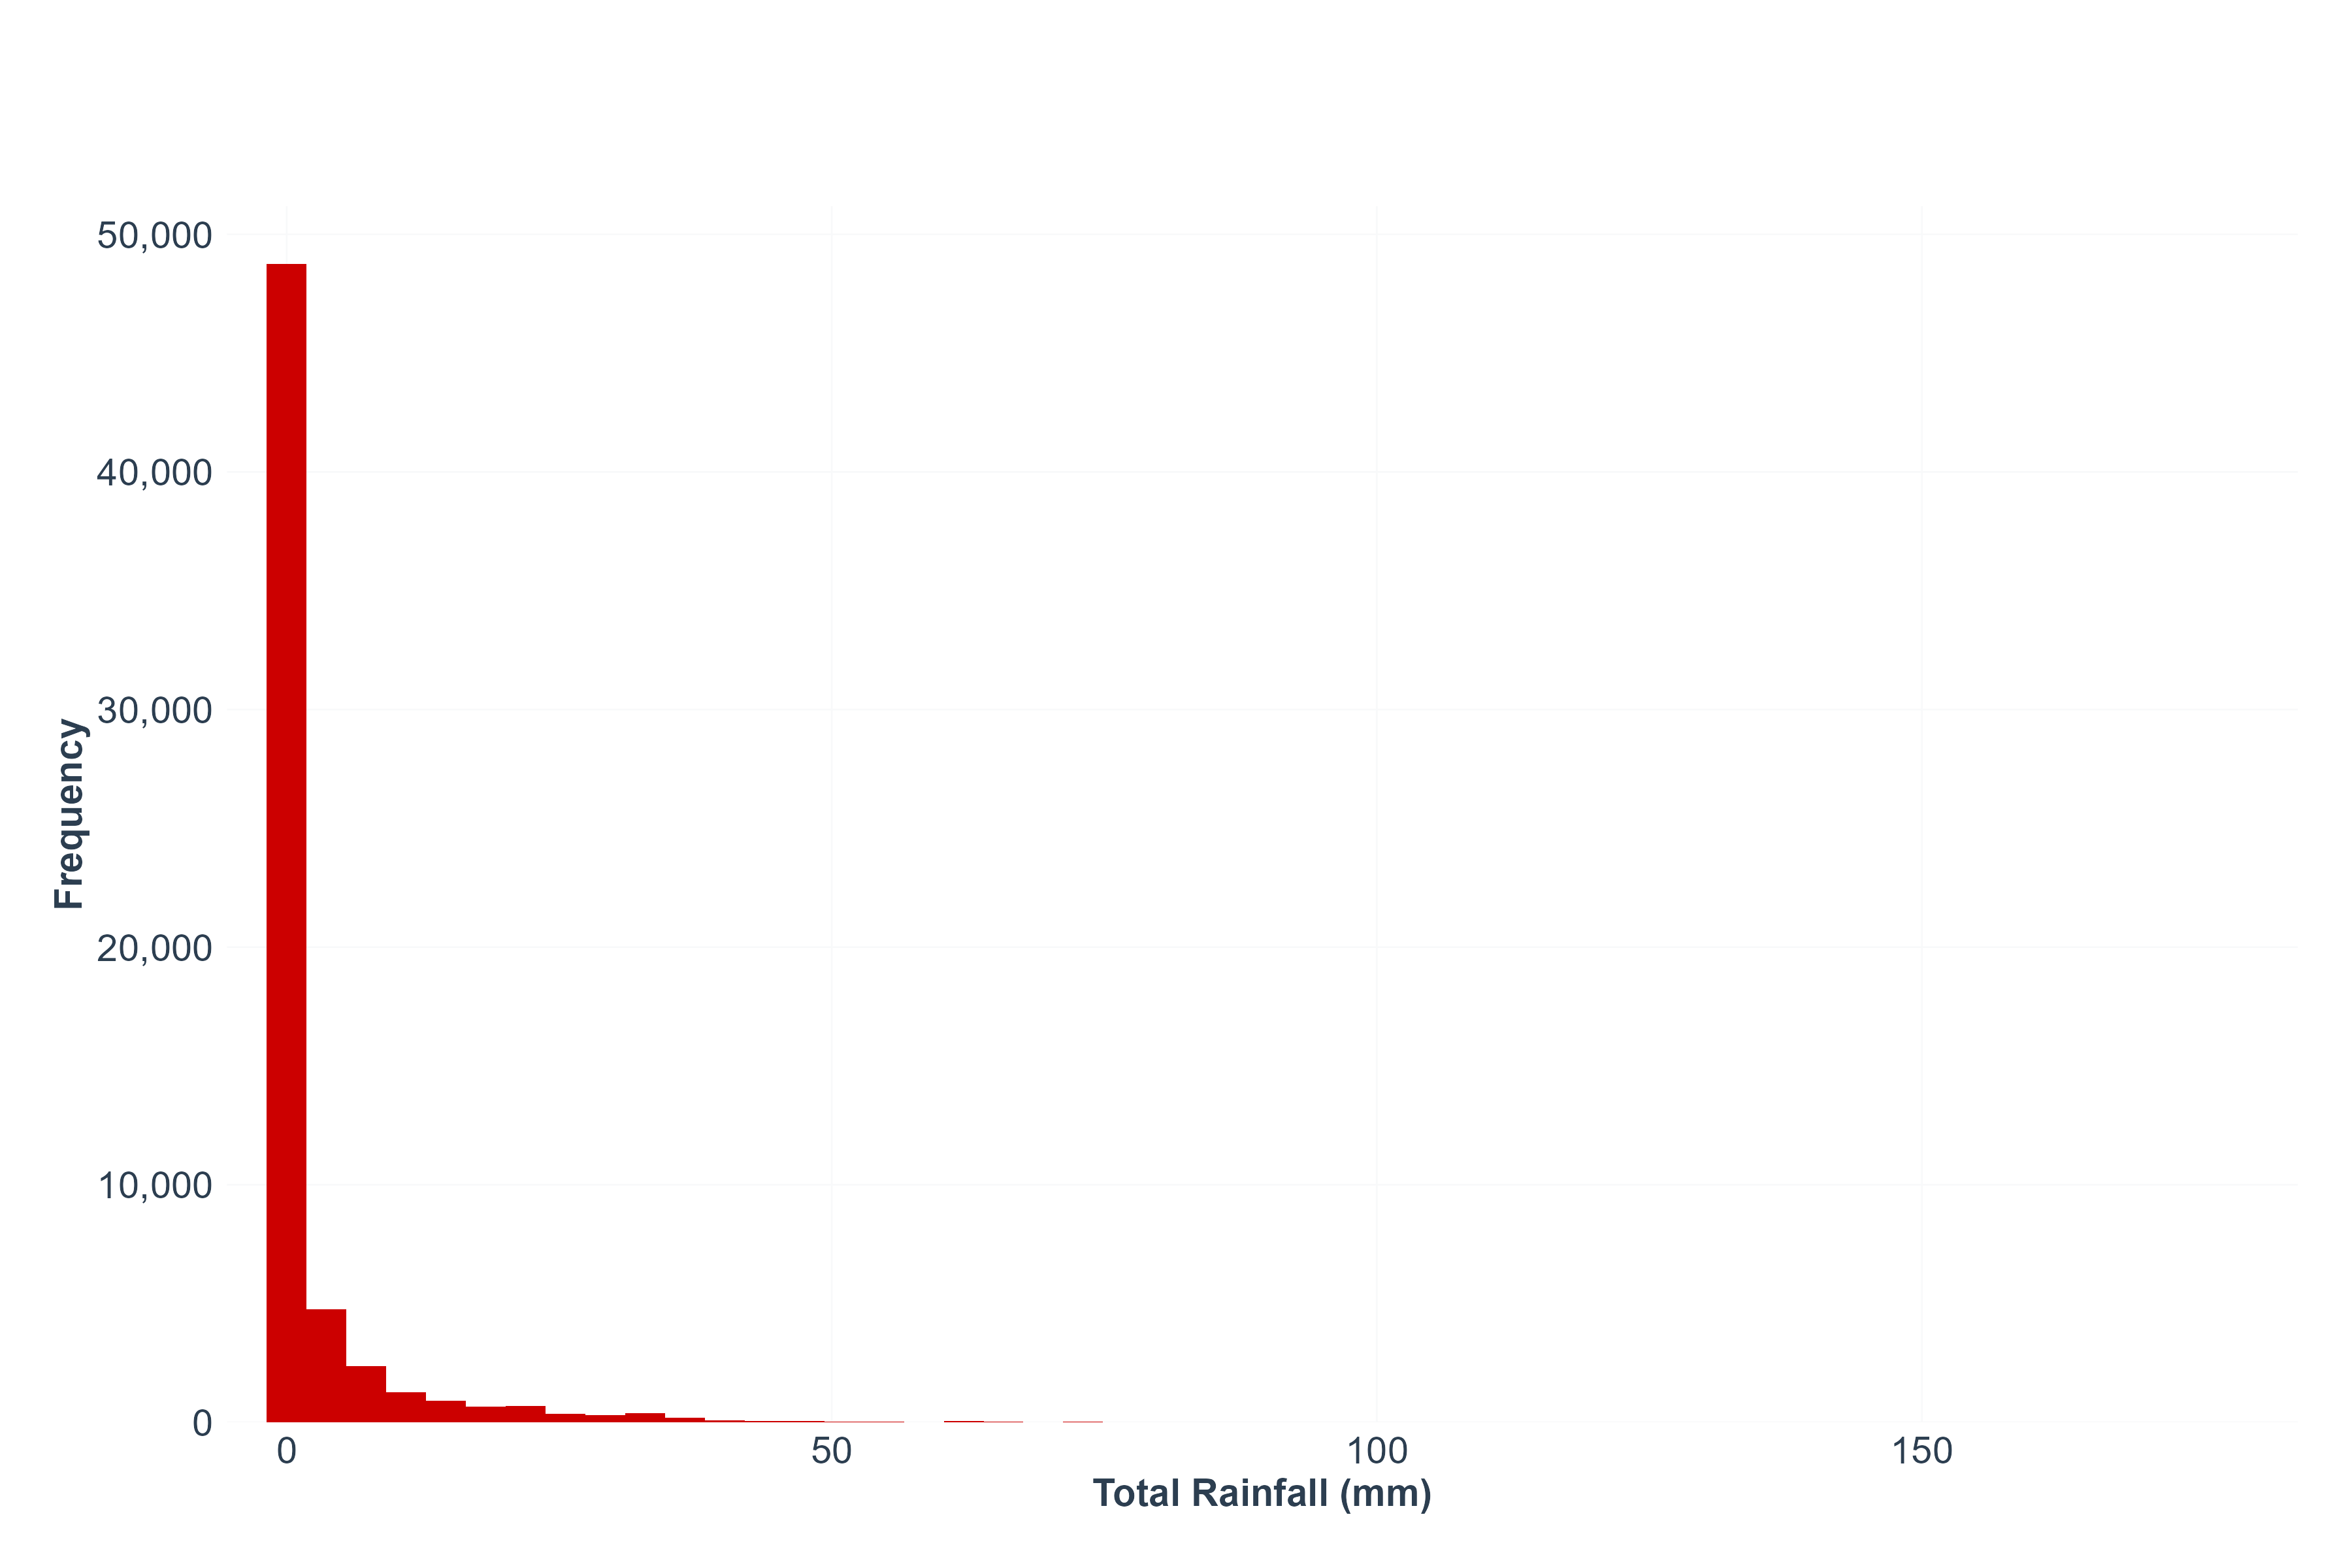
\includegraphics[width=0.8\textwidth]{../figures/rainfall_histogram.png}
    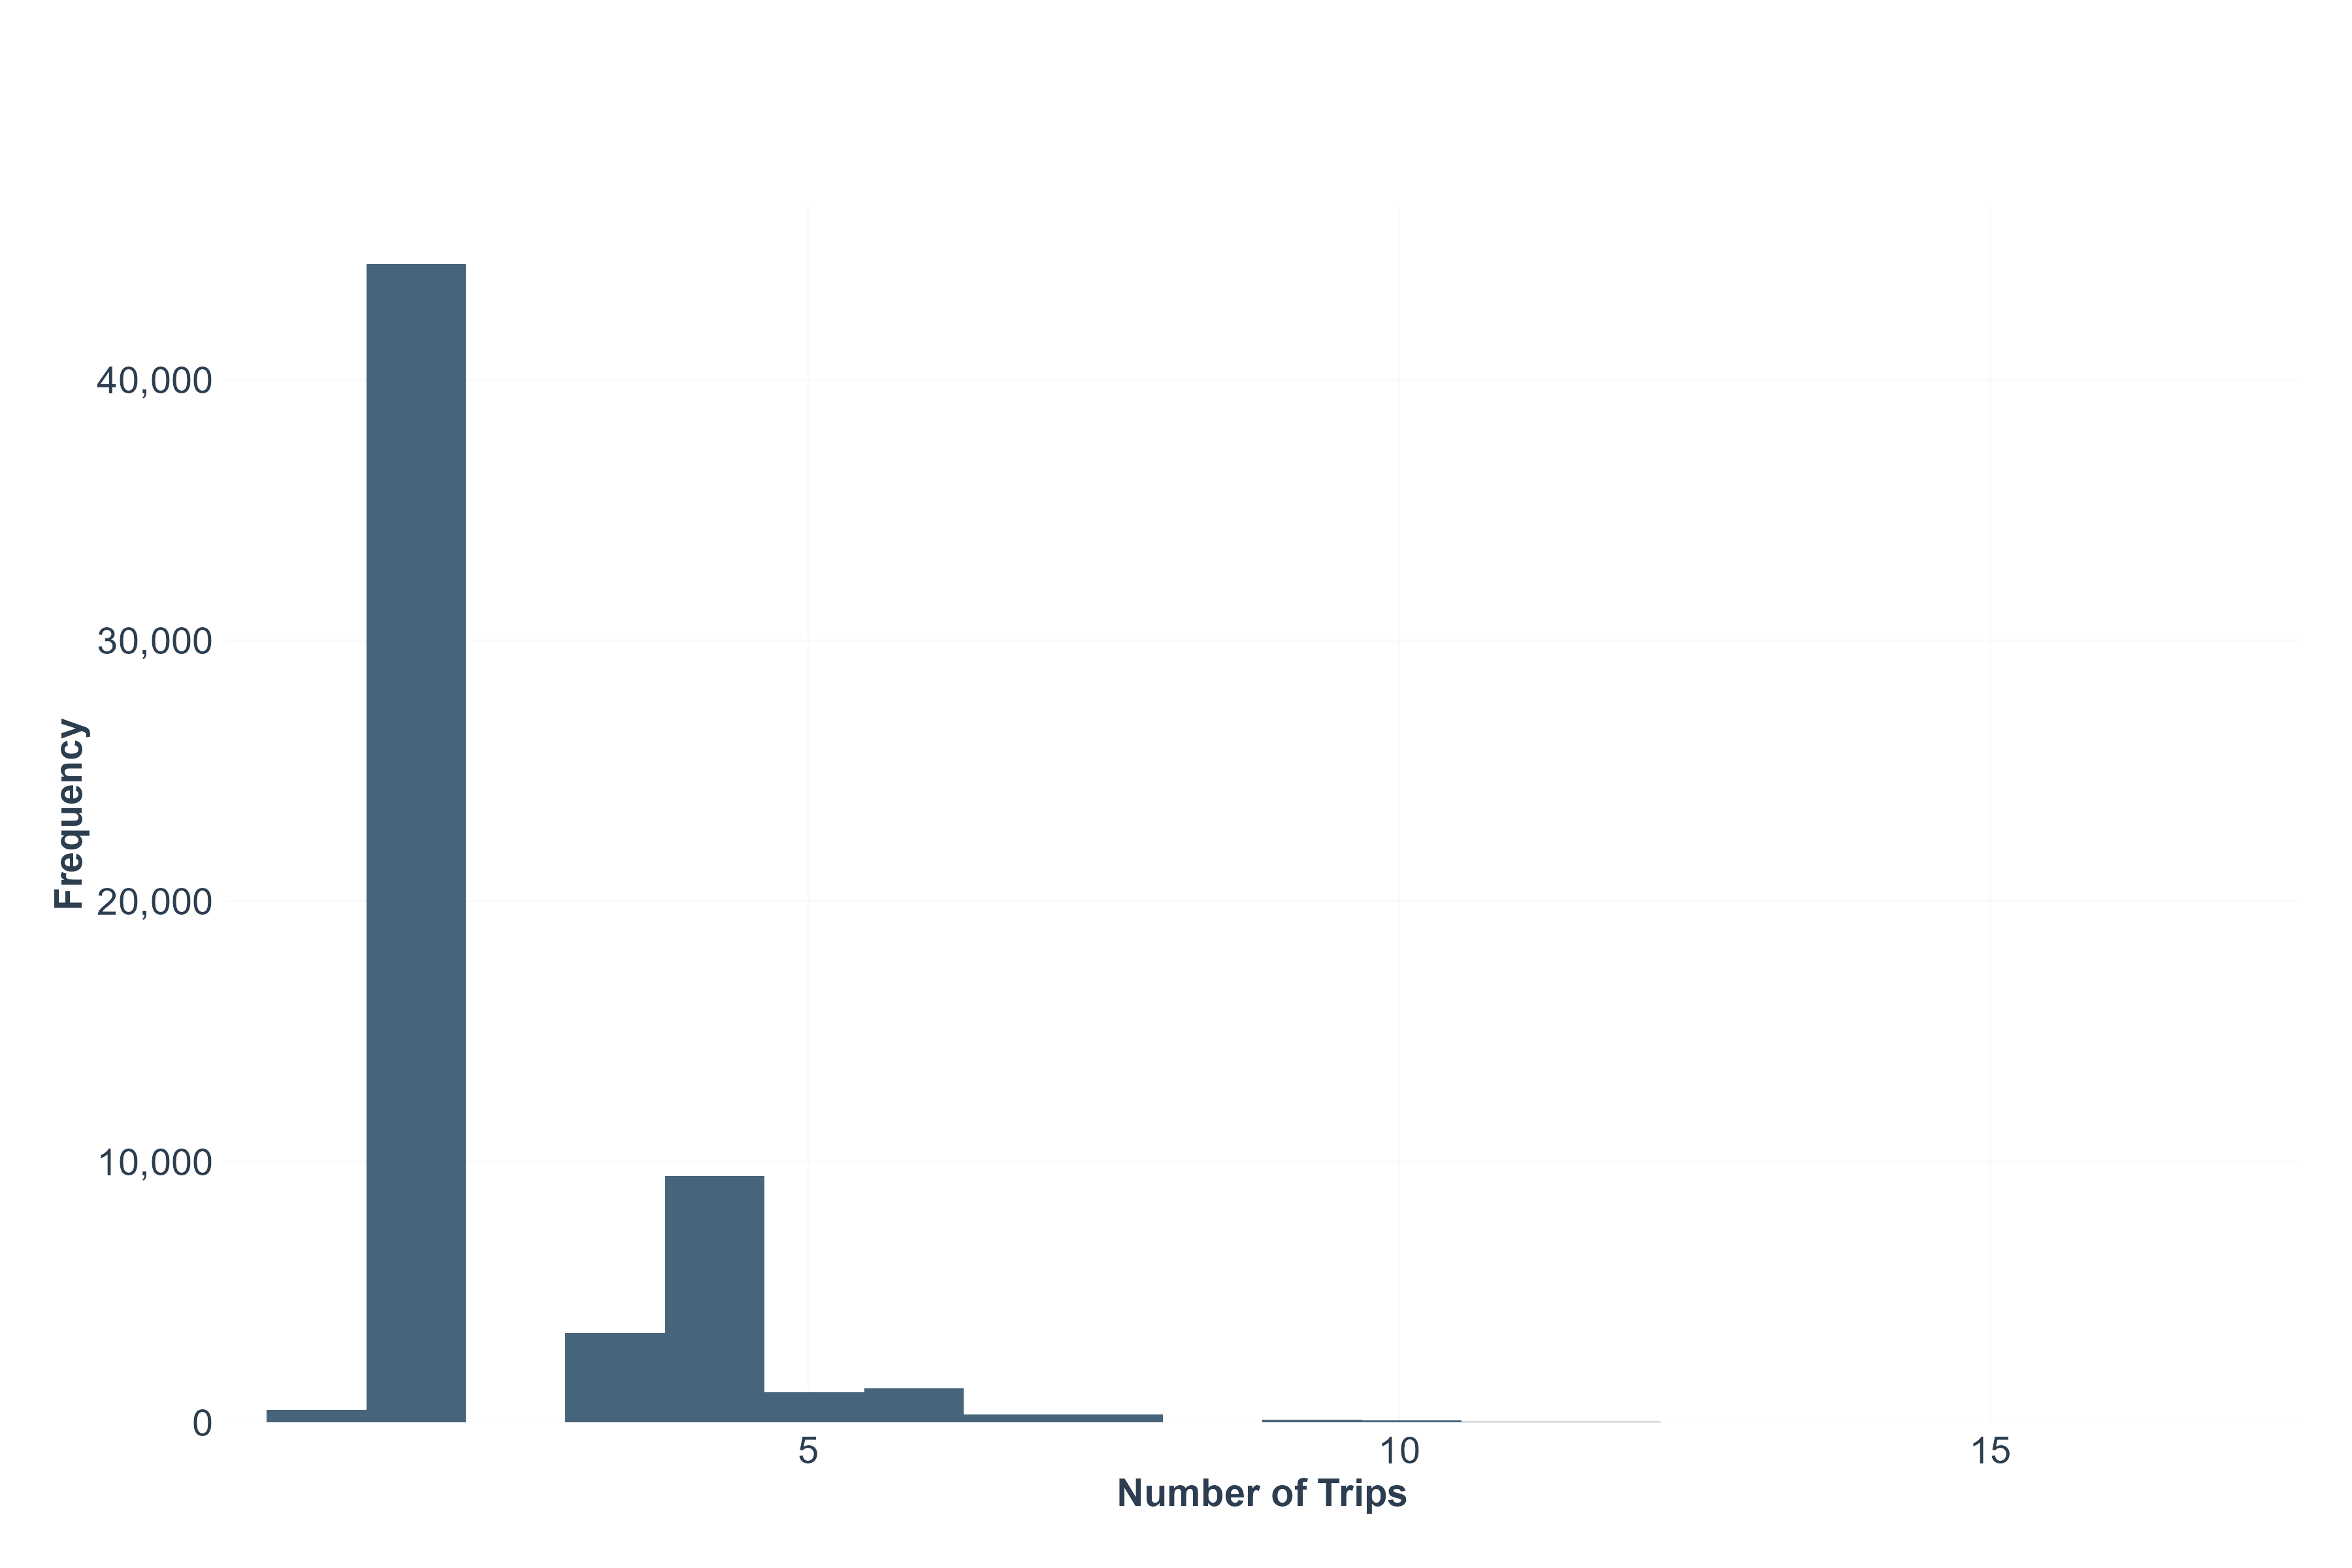
\includegraphics[width=0.8\textwidth]{../figures/trips_histogram.png}
    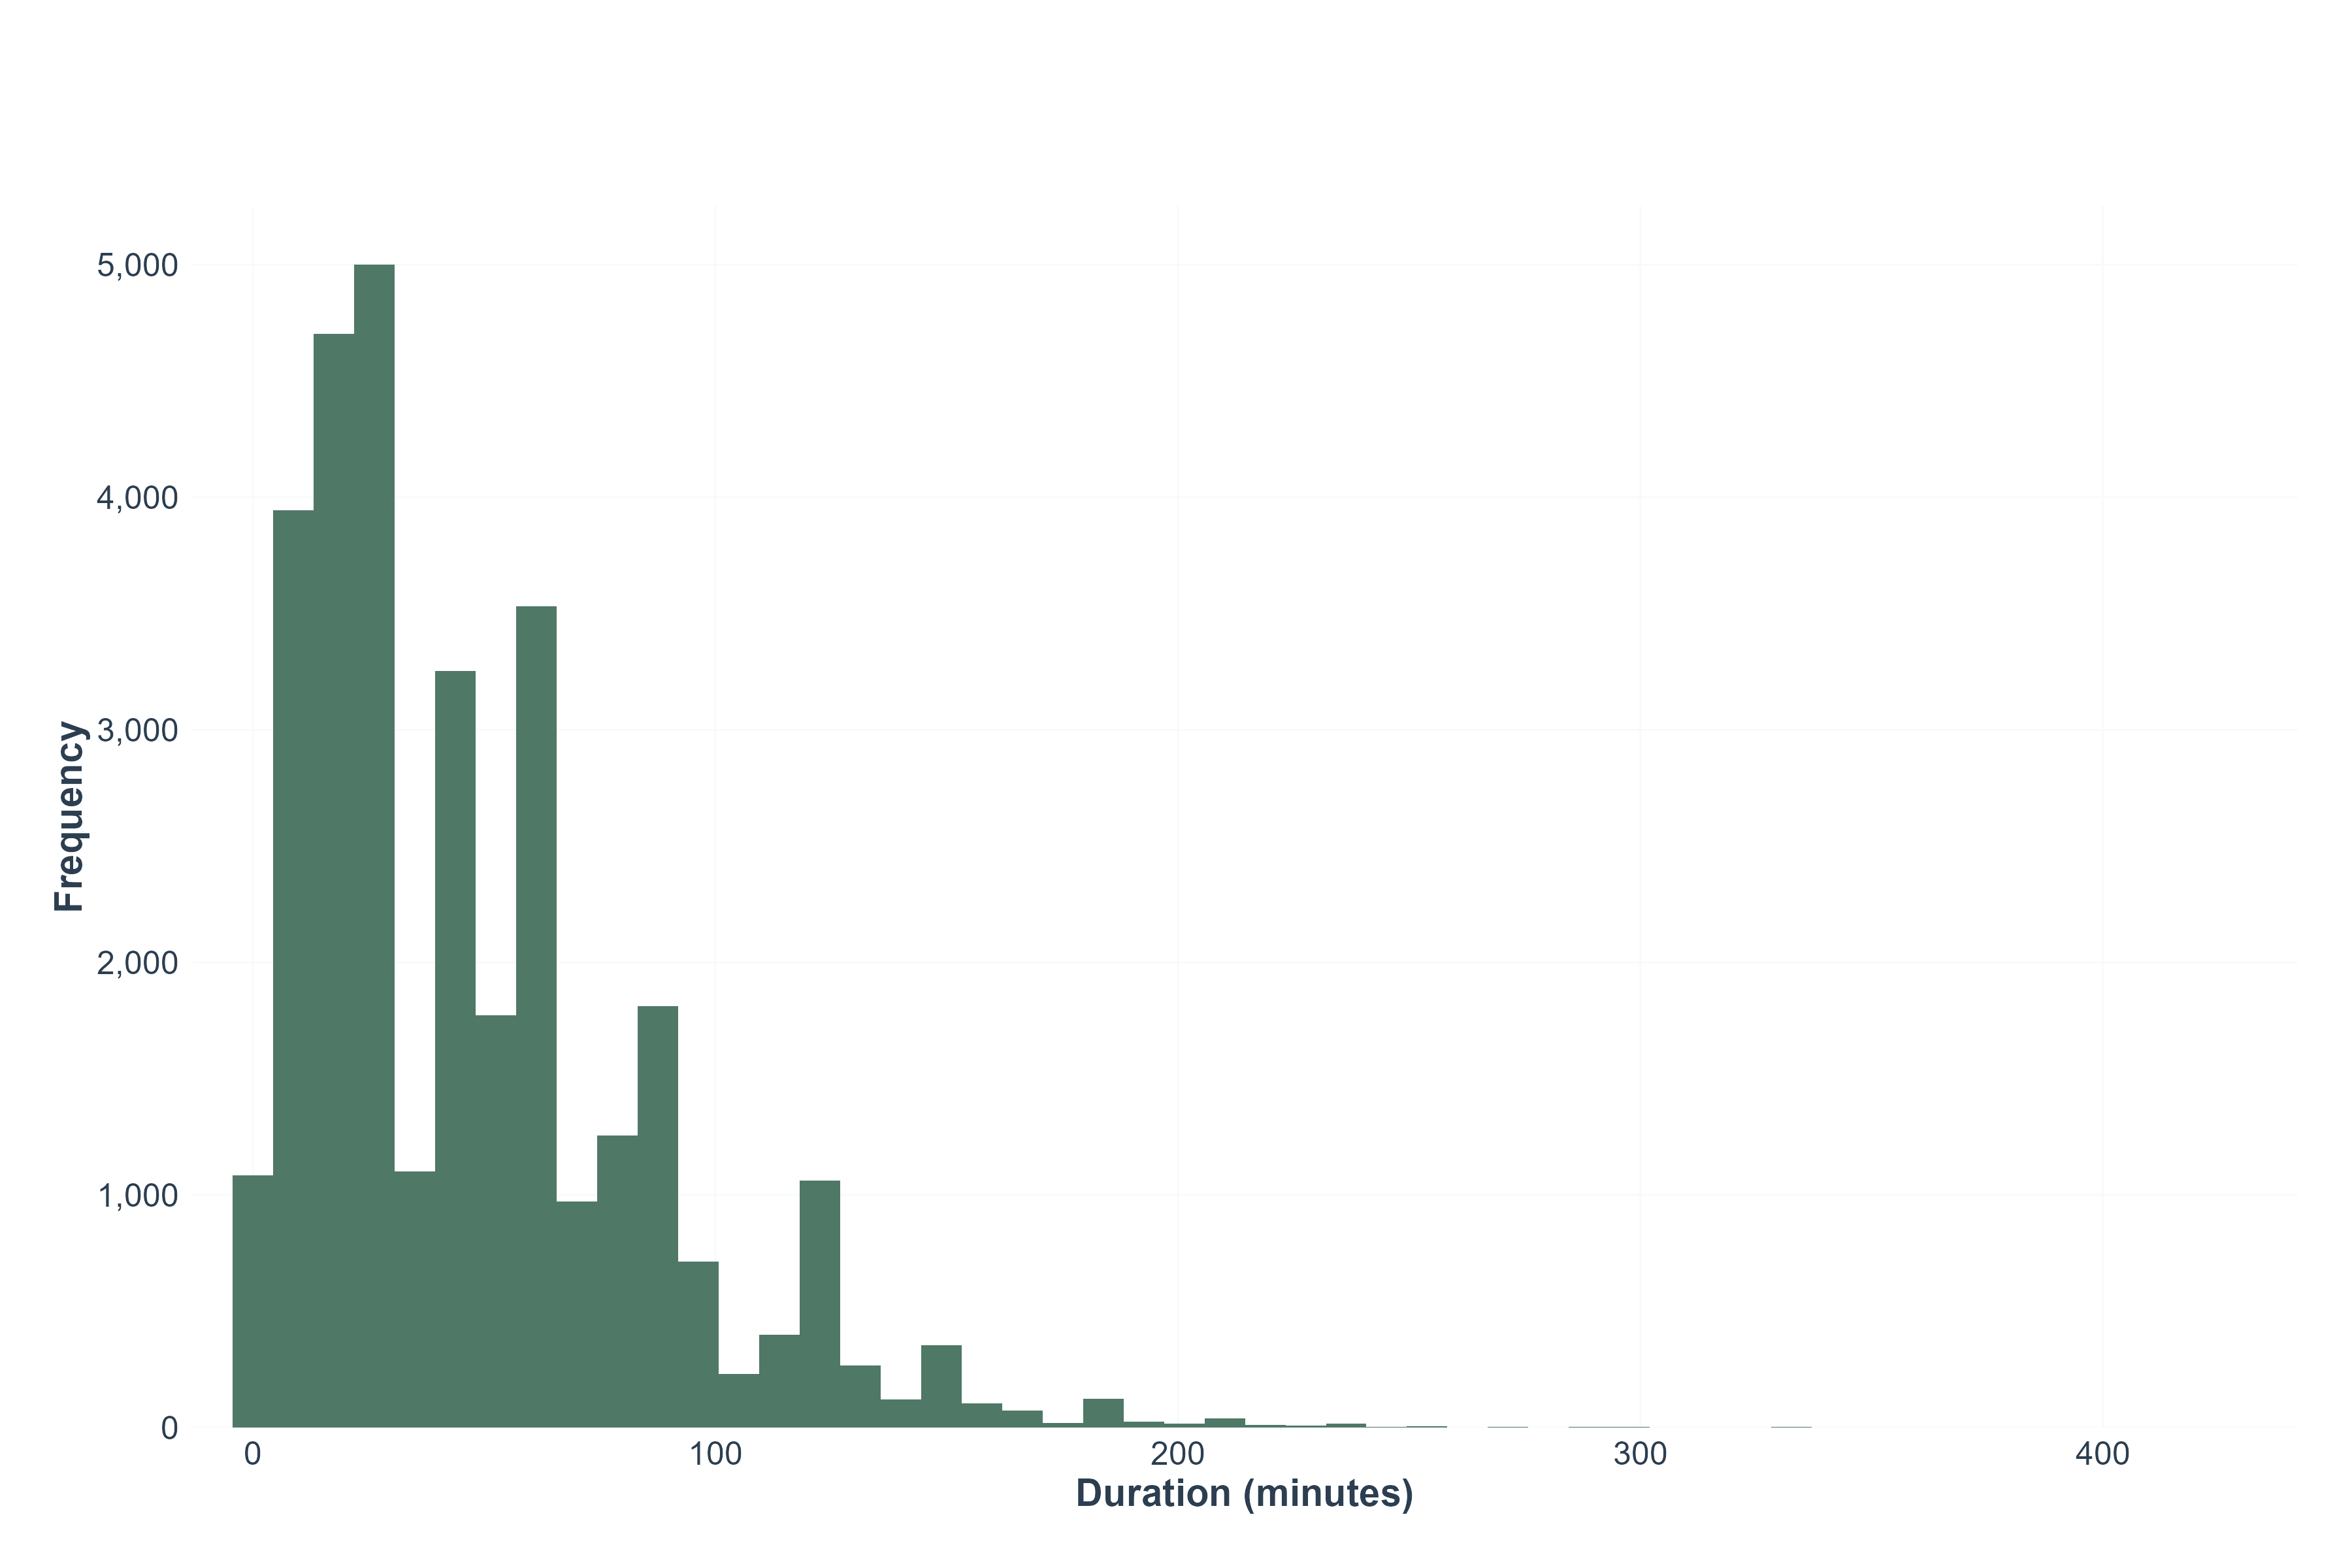
\includegraphics[width=0.8\textwidth]{../figures/duration_histogram.png}
    \caption{Histograms showing the distributions of rainfall (top), number of trips (middle), and commute durations (bottom) in the dataset.}
    \label{fig:hist}
\end{figure}

To combine the rainfall and labor market data, I developed a spatial matching procedure that links survey respondents to weather station measurements. I first calculated the geographic centroids of each origin-destination zone in the survey using municipal boundaries and zone definitions. Next, I created Voronoi polygons around each CEMADEN weather station, which partition the metropolitan area such that each location is assigned to its nearest weather station. I then matched each survey respondent's zone centroid to the corresponding weather station, assigning them the rainfall measurements from their nearest station. This approach ensures that each individual receives rainfall data from the most geographically relevant weather station while maintaining the spatial precision necessary for causal identification. The matching process accounts for the irregular spatial distribution of weather stations and survey zones. Figure \ref{fig:rmsp_voronoi} illustrates my spatial matching strategy, showing both the RMSP zone partitions and the Voronoi diagram I constructed.

\begin{figure}
    \centering
    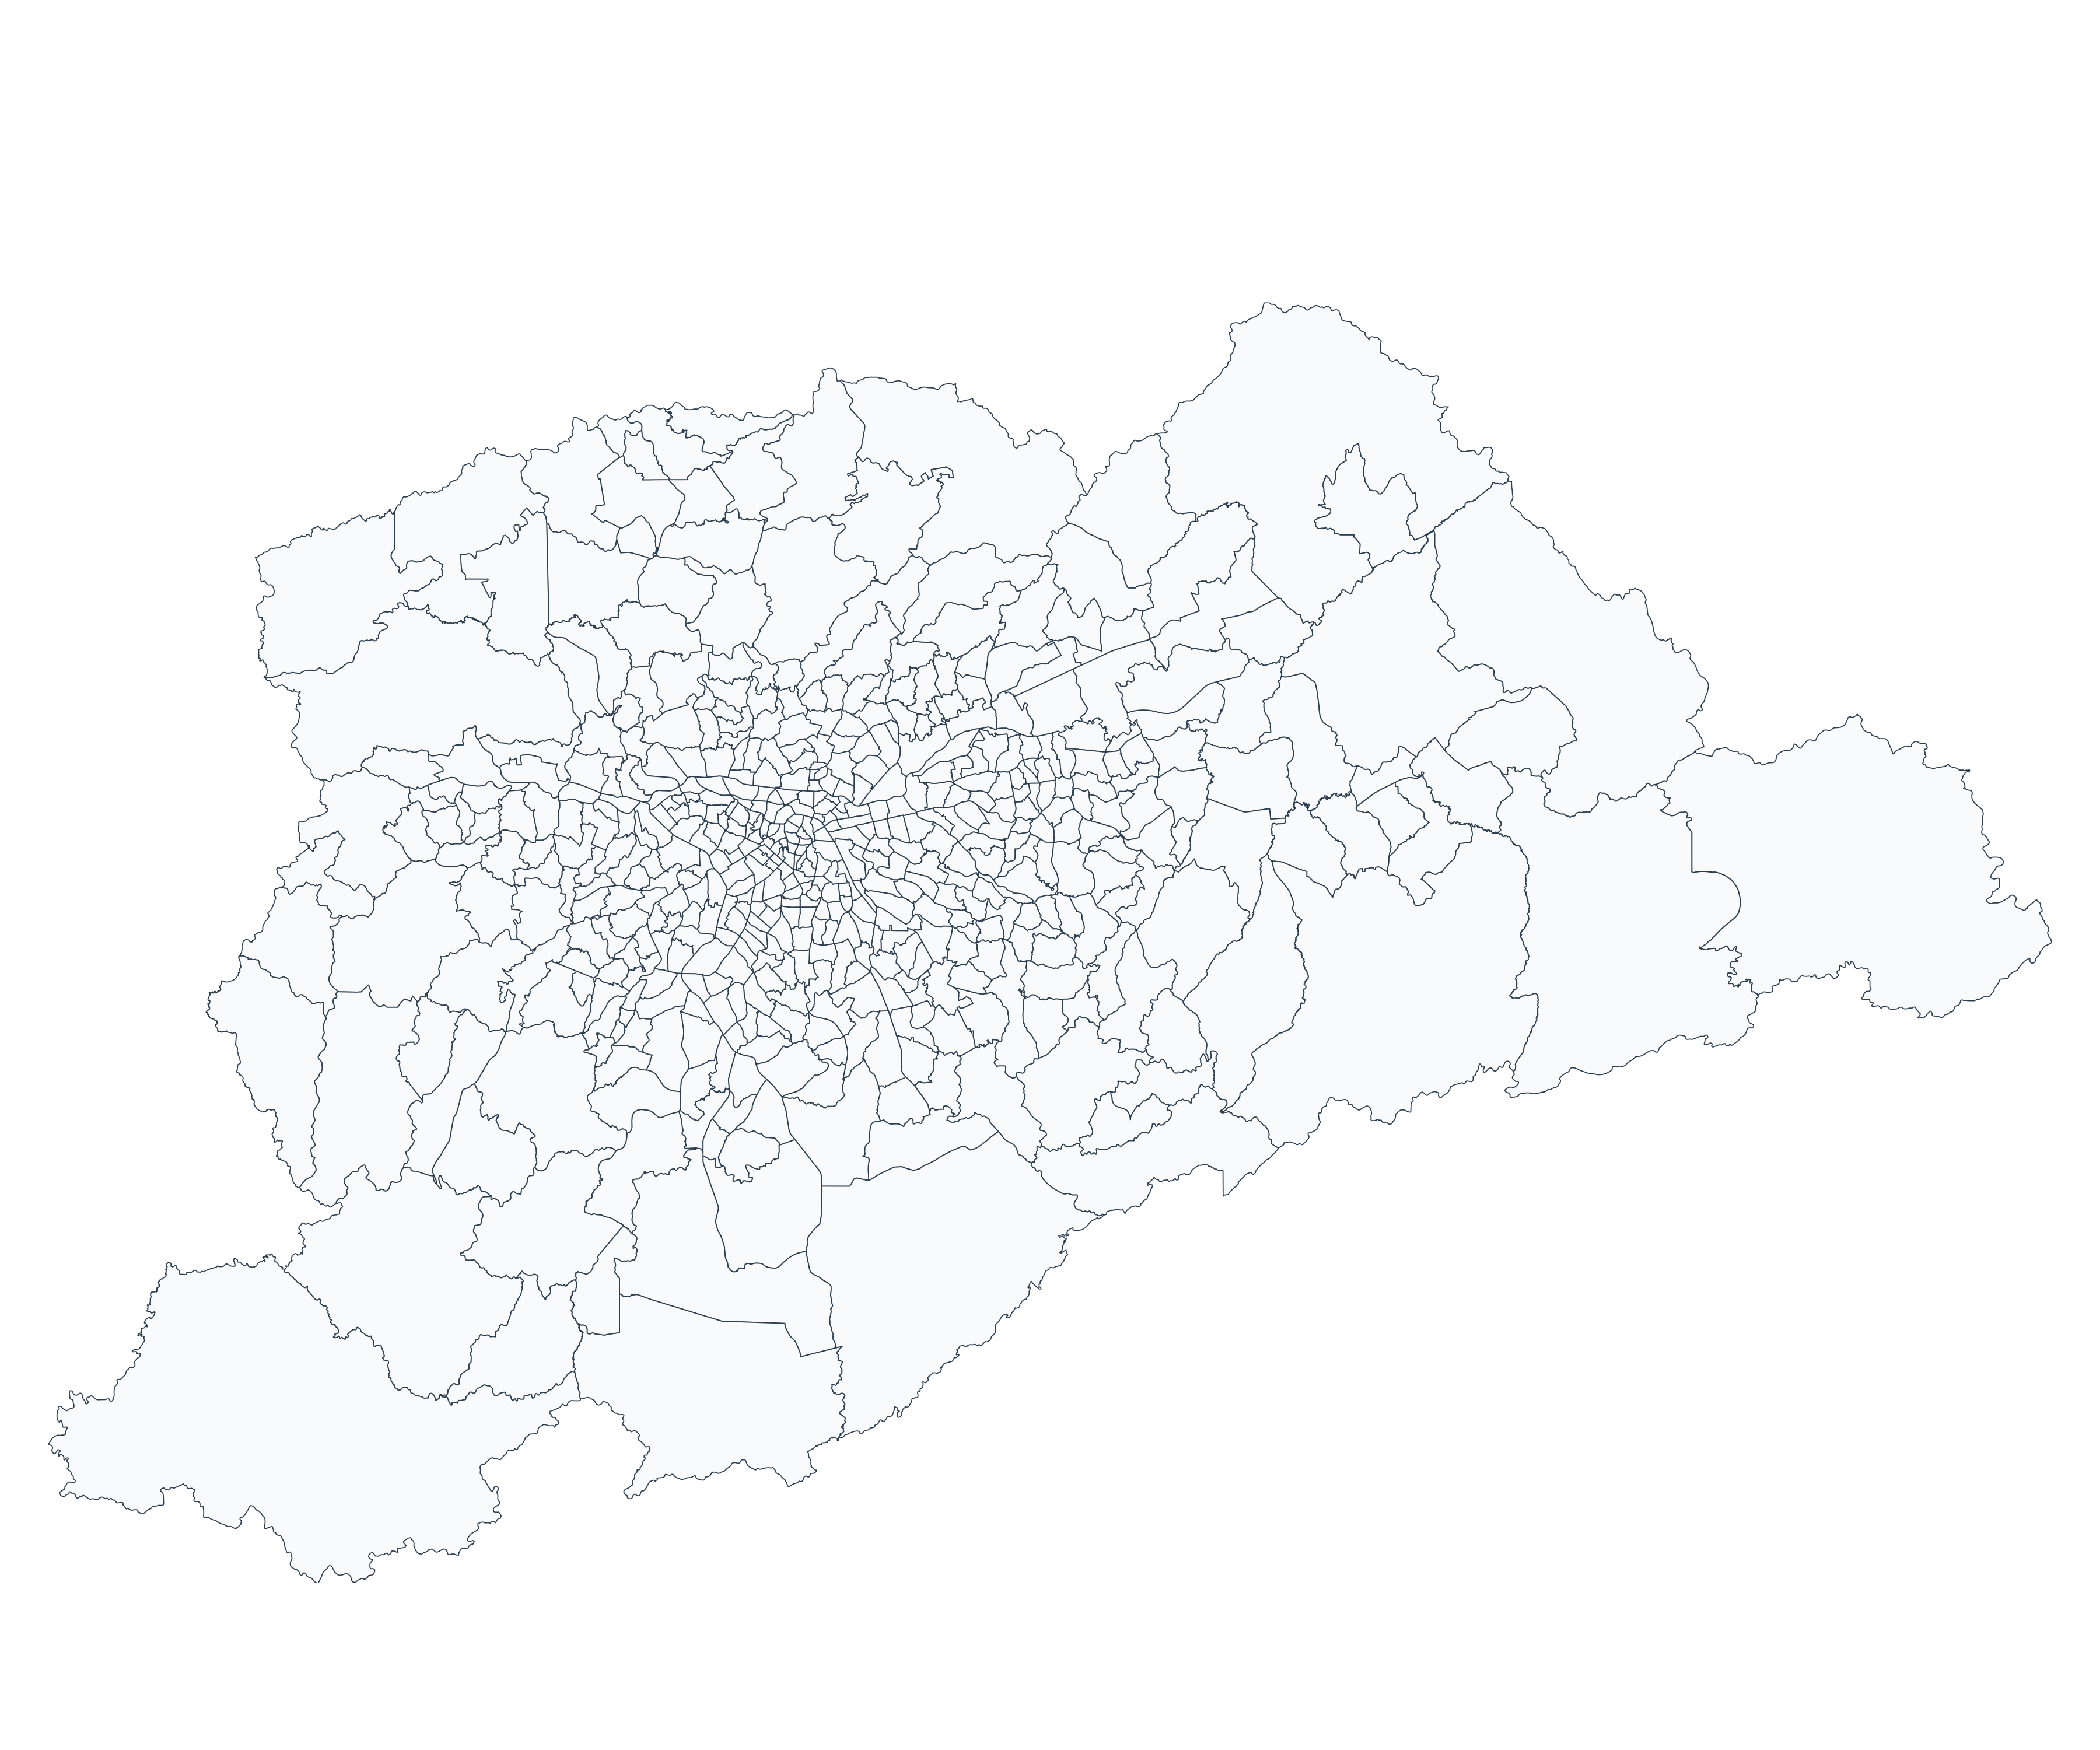
\includegraphics[width=0.8\textwidth]{../figures/rmsp_base.png}
    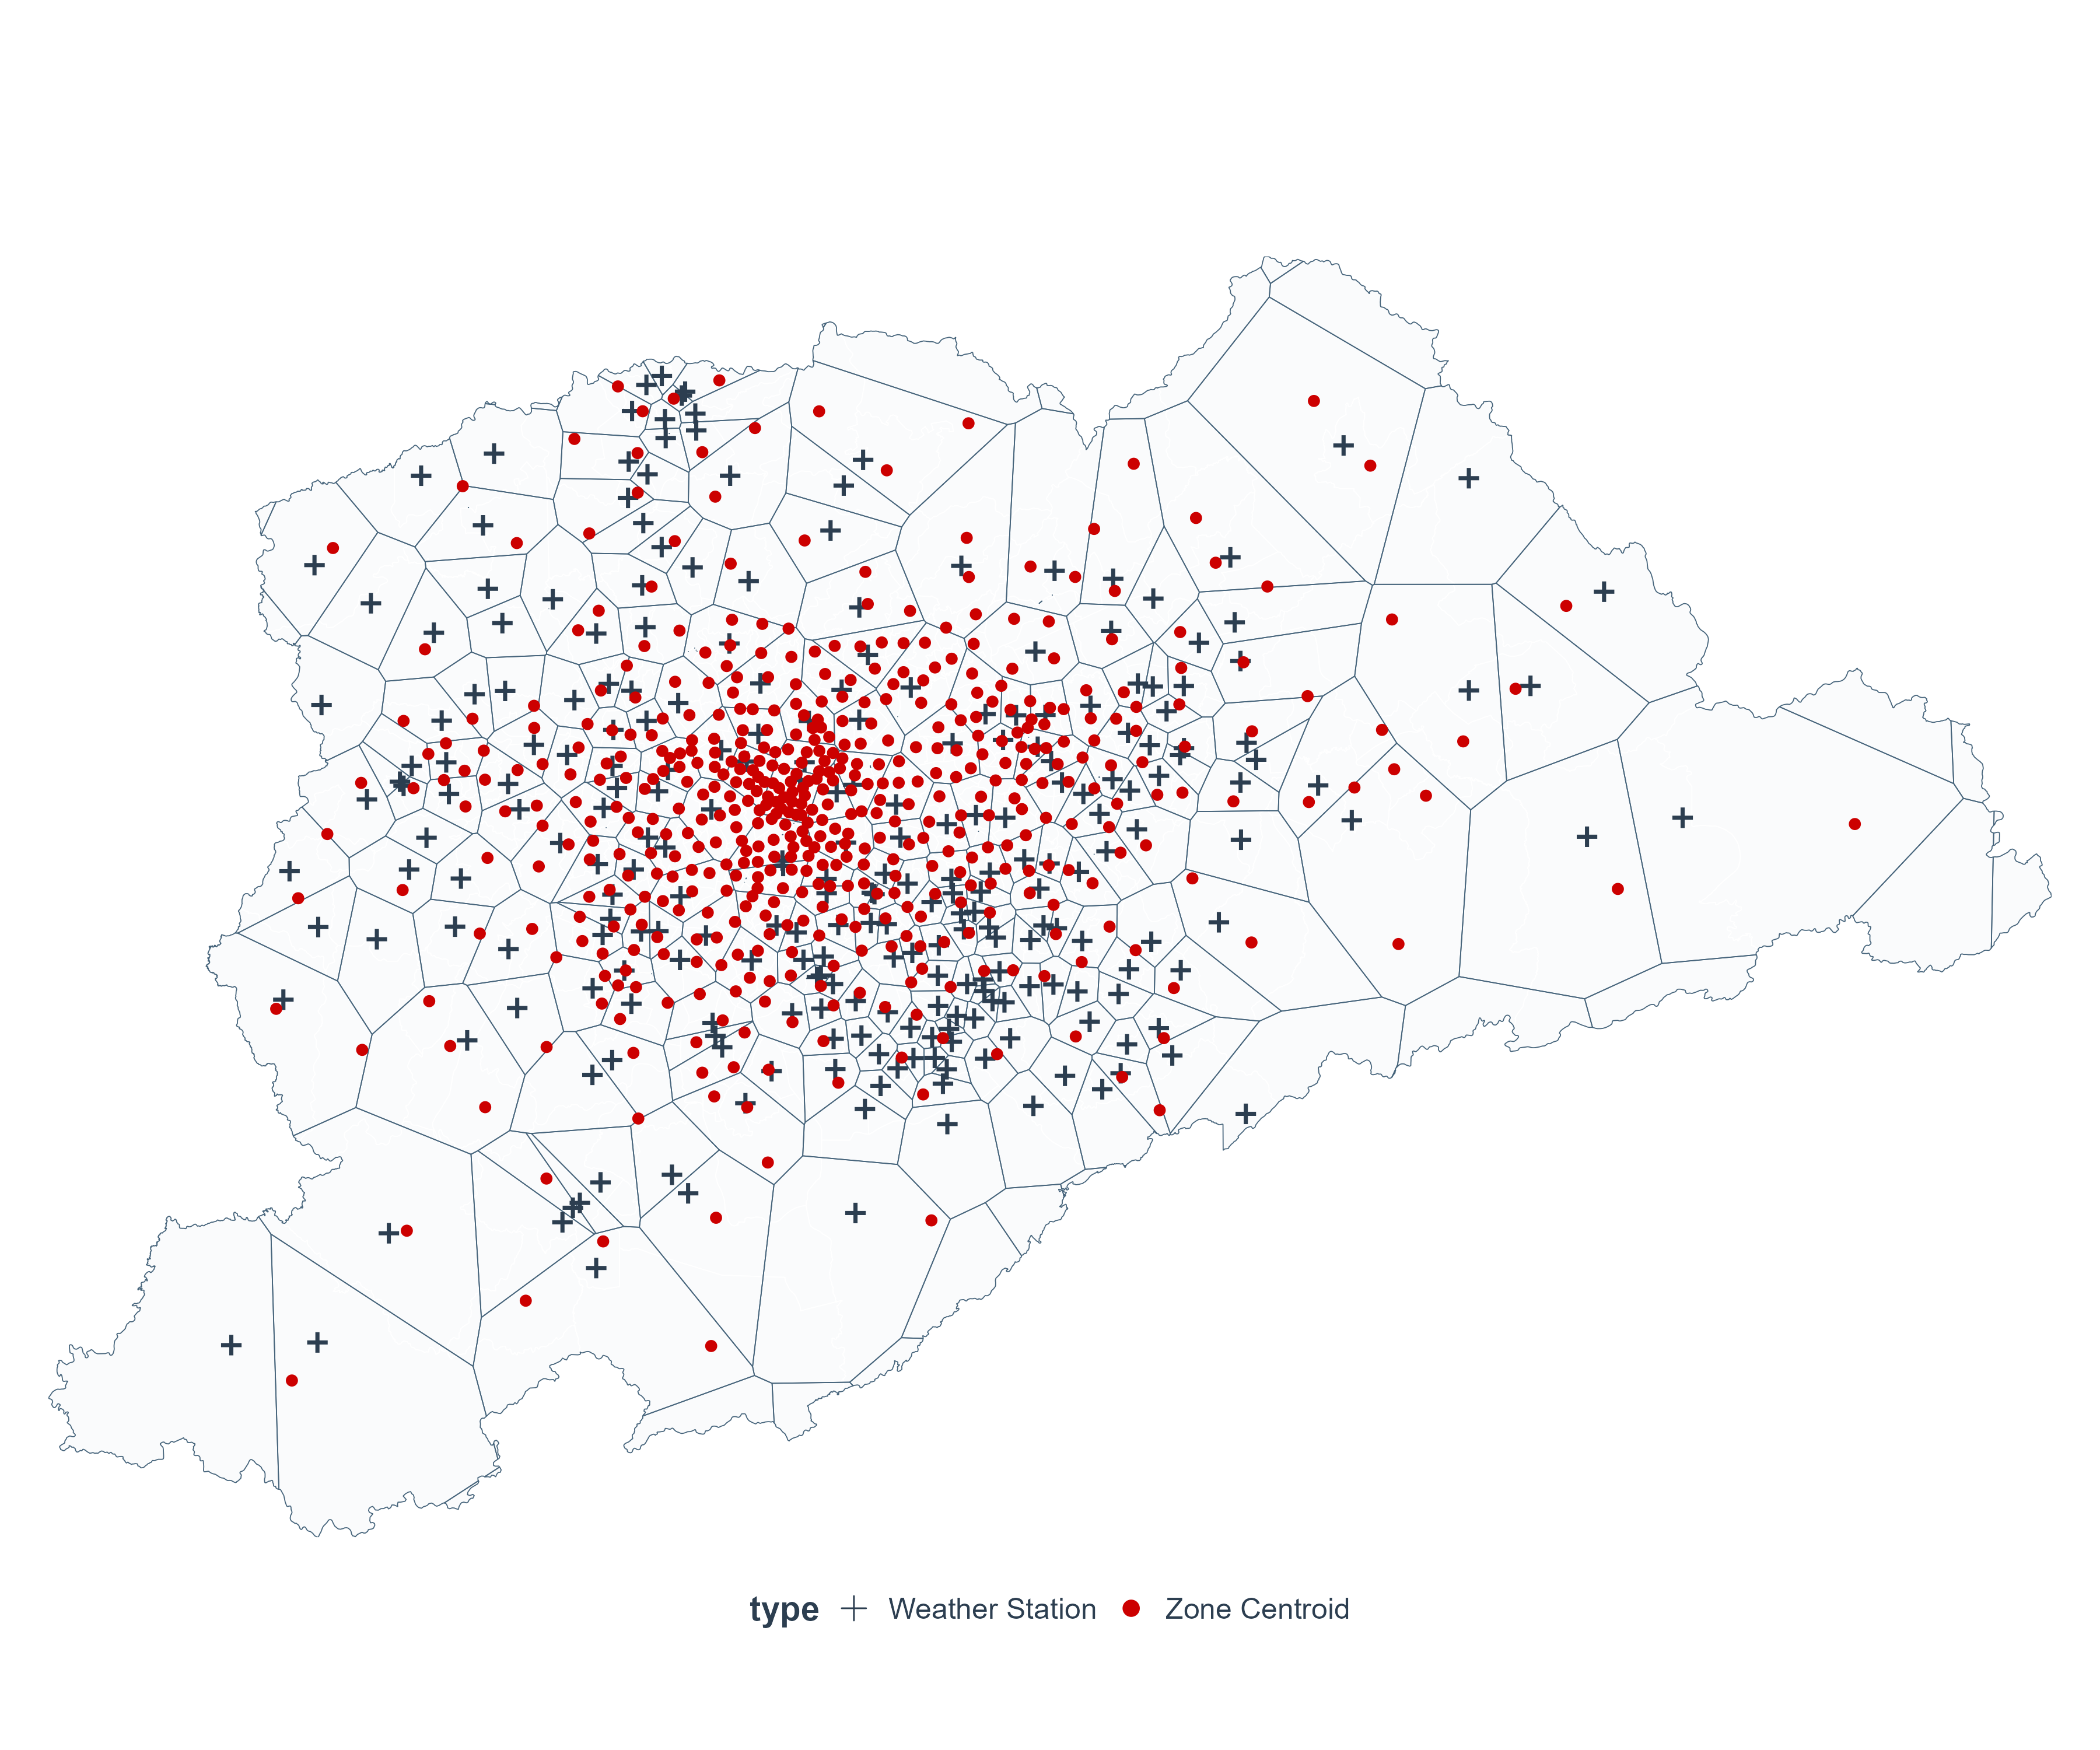
\includegraphics[width=0.8\textwidth]{../figures/rmsp_voronoi.png}
    \caption{Spatial representation of the RMSP region: (top) zone partitions, (bottom) Voronoi diagram illustrating spatial partitions based on centroid proximity to weather stations.}
    \label{fig:rmsp_voronoi}
\end{figure}

I employ a reduced-form approach that exploits plausibly exogenous variation in daily rainfall to identify causal effects on labor supply. I estimate the following models for work probability and commute time:
\begin{align*}
Y_{izt} &= \alpha + \beta_1 \text{Rain}_{izt} + \beta_2 \text{Rainfall}_{izt} + \mathbf{X}_{izt}'\gamma + \delta_z + u_{izt}
\end{align*}
where $Y_{izt}$ represents either a binary work indicator or commute time for individual $i$ in zone $z$ on reference day $t$, $\text{Rain}_{izt}$ is a dummy for any precipitation, $\text{Rainfall}_{izt}$ is total rainfall in millimeters, $\mathbf{X}_{izt}$ includes individual controls, and $\delta_z$ represents zone fixed effects. I do not exploit the temporal dimension of the data, because I do not have a panel setting, only to variation coming from different survey days. I estimate five specifications with progressively more controls: rainfall dummy only, rainfall amount only, both rainfall variables, both plus individual controls, and the full specification with zone fixed effects. The identifying assumption is that daily rainfall variation is exogenous to individual labor supply decisions, which is plausible given the short-term nature of weather variation and the difficulty of perfectly predicting daily precipitation.

My empirical analysis reveals null effects of rainfall on both the extensive and intensive margins of labor supply in the RMSP. For work probability, the estimated effect of rainfall is zero across all model specifications, indicating no impact of precipitation on the likelihood of working. For commute time, rainfall does not increase travel duration; in fact, the point estimate is negative and statistically significant in some specifications, suggesting a small reduction in commute time on rainy days. However, these effects are not robust across all models and are not economically meaningful. Overall, I find no evidence that rainfall affects either the probability of working or the duration of work-related commutes, as shown in Tables \ref{tab:panel_a} and \ref{tab:panel_b}.

\label{tab:panel_a}
\begin{table}
\centering
\begin{talltblr}[         %% tabularray outer open
caption={Effect of Rainfall on Work Probability},
note{}={* p \num{< 0.1}, ** p \num{< 0.05}, *** p \num{< 0.01}},
note{ }={Sample consists of individuals regularly employed or do side gigs who worked on reference day. The dependent variable is a binary indicator equal to 1 if the individual worked on the reference day, 0 otherwise. Individual controls include age, gender dummy, education level, activity status, occupation, economic sector, and employment type. Zone fixed effects control for time-invariant spatial characteristics. Standard errors are heteroskedasticity-robust (HC1) and are shown in parentheses.},
]                     %% tabularray outer close
{                     %% tabularray inner open
colspec={Q[]Q[]Q[]Q[]Q[]Q[]},
column{2,3,4,5,6}={}{halign=c,},
column{1}={}{halign=l,},
hline{6}={1,2,3,4,5,6}{solid, black, 0.05em},
}                     %% tabularray inner close
\toprule
& Model 1 & Model 2 & Model 3 & Model 4 & Model 5 \\ \midrule %% TinyTableHeader
Rain Dummy (>0mm) & \num{-0.004} &  & \num{-0.004} & \num{-0.003} & \num{-0.001} \\
& (\num{0.003}) &  & (\num{0.004}) & (\num{0.004}) & (\num{0.004}) \\
Total Rainfall (mm) &  & \num{-0.000} & \num{0.000} & \num{-0.000} & \num{-0.000} \\
&  & (\num{0.000}) & (\num{0.000}) & (\num{0.000}) & (\num{0.000}) \\
Num.Obs. & \num{35488} & \num{35488} & \num{35488} & \num{35482} & \num{35482} \\
Individual Controls & No & No & No & Yes & Yes \\
Zone Fixed Effects & No & No & No & No & Yes \\
\bottomrule
\end{talltblr}

\end{table}

\label{tab:panel_b}
\begin{table}
\centering
\begin{talltblr}[         %% tabularray outer open
caption={Effect of Rainfall on Commute Duration},
note{}={* p \num{< 0.1}, ** p \num{< 0.05}, *** p \num{< 0.01}},
note{ }={Sample consists of individuals regularly employed or do side gigs who worked on reference day. The dependent variable is commute duration in minutes. Individual controls include age, gender dummy, education level, activity status, occupation, economic sector, and employment type. Zone fixed effects control for time-invariant spatial characteristics. Standard errors are heteroskedasticity-robust (HC1) and are shown in parentheses.},
]                     %% tabularray outer close
{                     %% tabularray inner open
colspec={Q[]Q[]Q[]Q[]Q[]Q[]},
column{2,3,4,5,6}={}{halign=c,},
column{1}={}{halign=l,},
hline{6}={1,2,3,4,5,6}{solid, black, 0.05em},
}                     %% tabularray inner close
\toprule
& Model 1 & Model 2 & Model 3 & Model 4 & Model 5 \\ \midrule %% TinyTableHeader
Rain Dummy (>0mm) & \num{-0.925}** &  & \num{-0.864}* & \num{-0.295} & \num{-0.144} \\
& (\num{0.436}) &  & (\num{0.488}) & (\num{0.473}) & (\num{0.483}) \\
Total Rainfall (mm) &  & \num{-0.035} & \num{-0.009} & \num{-0.023} & \num{0.019} \\
&  & (\num{0.031}) & (\num{0.034}) & (\num{0.033}) & (\num{0.034}) \\
Num.Obs. & \num{31715} & \num{31715} & \num{31715} & \num{31711} & \num{31711} \\
Individual Controls & No & No & No & Yes & Yes \\
Zone Fixed Effects & No & No & No & No & Yes \\
\bottomrule
\end{talltblr}

\end{table}


These results indicate that daily rainfall variation does not substantially influence short-term labor supply decisions in this urban Brazilian context. The findings hold across different model specifications, including those with comprehensive individual controls and zone fixed effects, and suggest that neither the extensive effect nor the intensive effect significantly alters work behavior or commute times.  

There are several limitations to this analysis. First, the correlation of rainfall across different zones in Sao Paulo is high, so the identification relies primarily on between-day variation among different survey days rather than within-day variation. As the data covers only weekdays for a single year, this may limit the amount of variation in outcomes. Second, the analysis does not capture the effects of extreme weather events such as flooding, which may have more pronounced impacts on labor market outcomes and urban infrastructure. Future research could investigate the effects of such disasters, as well as explore heterogeneous impacts across formal and informal labor markets, or between central and peripheral urban areas.



% --- Bibliography ---
\newpage
\bibliography{references}
\bibliographystyle{chicago}


% --- Document ends here ---

\end{document}
